\chapter{Marco Metodológico: Arquitectura General del Sistema}

Los algoritmos actuales de reconstrucción, como Multi View Stereo (MVS), operan bajo un paradigma de densificación exhaustiva. El problema principal de este enfoque es que resulta excesivamente costoso y redundante computacionalmente, ya que intenta densificar millones de píxeles sin entender la estructura de lo que está reconstruyendo. Generar estas nubes masivas se vuelve inmanejable para entornos urbanos a gran escala.

Para solucionar esto, el sistema propuesto plantea un modelo basado firmemente en la abstracción semántica y geométrica. En lugar de procesar a ciegas la profundidad, el enfoque busca comprender primero la escena arquitectónica para luego triangular únicamente las primitivas estructurales necesarias. 

Este capítulo presenta un resumen rápido y estructurado de las fases que conforman la arquitectura propuesta, delineando la idea general del proyecto. Los detalles matemáticos y la implementación técnica profunda de cada fase se abordarán con muchísimo detalle en los capítulos posteriores.

\section{Pipeline de Reconstrucción}
El \textit{pipeline} propuesto abandona por completo la densificación clásica basada en píxeles. Esto funciona dividiendo el problema en fases secuenciales, priorizando en todo momento la extracción de caras y fronteras arquitectónicas.

\subsection{Fase 1: Preprocesamiento y Enmascaramiento Dinámico}
Esta fase sirve para limpiar las secuencias de video de información no deseada. Funciona a través de modelos de inferencia rápida, como FastSAM o YOLO, los cuales detectan objetos dinámicos dentro de la escena (típicamente autos y peatones), tal como se ejemplifica en la Figura \ref{fig:yolo_masking}.

\begin{figure}[H]
    \centering
    \begin{minipage}{0.48\textwidth}
        \centering
        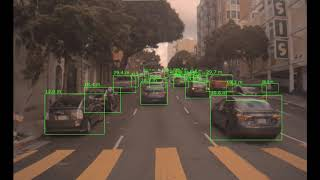
\includegraphics[width=\linewidth]{images/yolo_masking.png}
    \end{minipage}\hfill
    \begin{minipage}{0.48\textwidth}
        \centering
        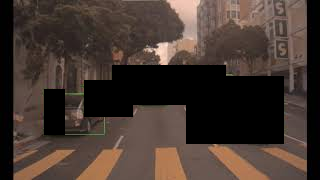
\includegraphics[width=\linewidth]{images/yolo_blacked.png}
    \end{minipage}
    \caption{Proceso de preprocesamiento: Identificación de elementos dinámicos con YOLO (izquierda) y su posterior enmascaramiento o censura espacial (derecha) para evitar ruido en la geometría (Fuente: Adaptado de \url{https://youtu.be/ftsUg5VlzIE}).}
    \label{fig:yolo_masking}
\end{figure}

Una vez identificados, se aplica un enmascaramiento dinámico (\textit{Masking}) para omitir estas regiones temporalmente de los cálculos geométricos. Un enfoque alternativo que muchos podrían sugerir es rellenar estos vacíos utilizando técnicas de \textit{Video Inpainting} previo a la reconstrucción. Sin embargo, como lo advierte la literatura en sistemas de mapeo dinámico \cite{bescos2018dynaslam}, la desventaja crítica del \textit{inpainting} generativo no es su tiempo de cómputo, sino su \textbf{inestabilidad geométrica}. 

Estos modelos \textit{alucinan} texturas visualmente plausibles pero carentes de consistencia temporal. Esta inestabilidad genera parpadeos y características falsas entre \textit{frames} que terminan corrompiendo de forma irremediable la geometría epipolar y el rastreo (\textit{tracking}) de la cámara.

\begin{itemize}
    \item \textbf{Resumen:} Se usan modelos de segmentación rápida para enmascarar y descartar los objetos móviles, optando por ignorar la información en lugar de inventarla con \textit{inpainting}, salvaguardando así la pureza matemática del sistema.
\end{itemize}

\subsection{Fase 2: Extracción Estructural y Tracking Híbrido}
El objetivo de esta fase es rastrear la trayectoria de la cámara y obtener la estructura base evadiendo los descriptores clásicos basados en texturas, como SIFT o ORB, porque son propensos a fallar en entornos repetitivos o sin textura. 

Se utilizan arquitecturas neuronales de última generación, como Co-PLNet \cite{wang2026coplnet}, para extraer nodos clave y los \textit{wireframes} estructurales en cada imagen. Como se observa en la Figura \ref{fig:coplnet_examples}, la red identifica con precisión las esquinas y líneas arquitectónicas de la edificación. 

\begin{figure}[H]
    \centering
    \begin{minipage}{0.48\textwidth}
        \centering
        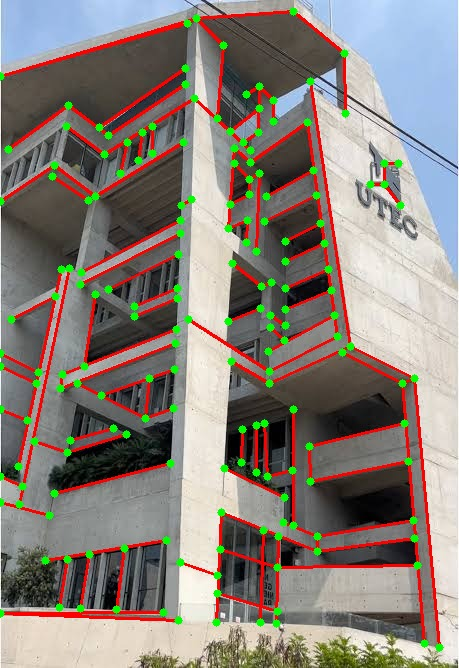
\includegraphics[width=\linewidth]{images/coplnet_utec1.png}
    \end{minipage}\hfill
    \begin{minipage}{0.48\textwidth}
        \centering
        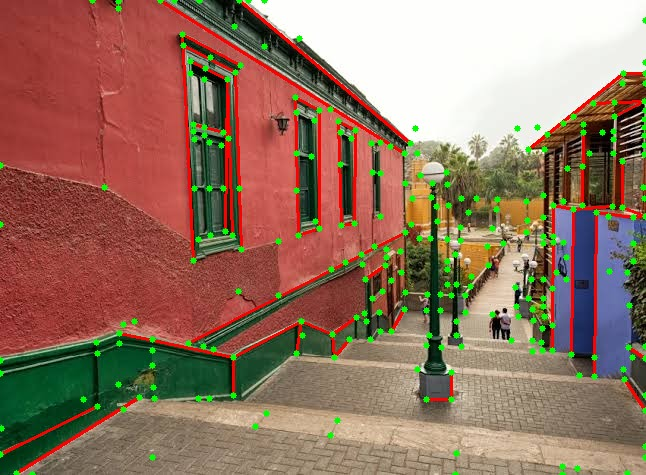
\includegraphics[width=\linewidth]{images/coplnet_barranco.png}
    \end{minipage}
    \caption{Demostración de extracción conjunta de puntos y líneas sobre edificaciones reales utilizando Co-PLNet. Se observan los nodos estructurales en verde y las fronteras arquitectónicas en rojo (Fuente: Elaboración propia).}
    \label{fig:coplnet_examples}
\end{figure}

Posteriormente, se aplican arquitecturas de grafos, específicamente GlueStick \cite{pelaez2023gluestick}, para realizar un emparejamiento robusto conjunto de puntos y líneas. Esto permite calcular una triangulación dispersa inicial que estima la pose de la cámara.

\subsection{Fase 3: Segmentación y Detección de Caras (Planos)}
En esta etapa, el sistema inyecta restricciones semánticas para detectar y segmentar los planos arquitectónicos dominantes usando modelos especializados como ZeroPlane \cite{liu2025zeroplane}, PlaneRCNN \cite{liu2019planercnn}, o combinaciones robustas usando DUSt3R \cite{wang2024dust3r} y SAM. Como se ejemplifica en la Figura \ref{fig:plane_segmentation}, estas arquitecturas son capaces de identificar y aislar matemáticamente las distintas instancias planas que componen la escena.

\begin{figure}[H]
    \centering
    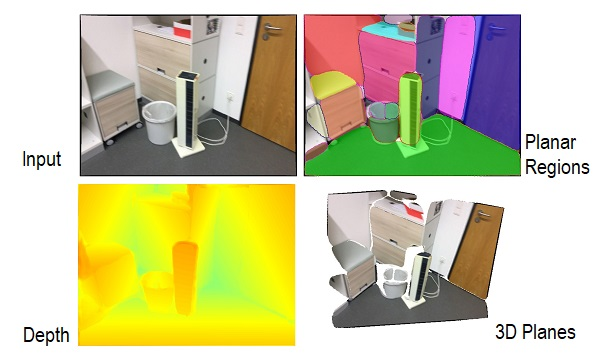
\includegraphics[width=0.95\textwidth]{images/planercnn_segmentation.jpg}
    \caption{Demostración de segmentación de superficies planares. La imagen ilustra cómo la red infiere máscaras para cada instancia plana detectada. Cada color representa un plano geométrico distinto, facilitando la distinción entre superficies arquitectónicas y elementos ajenos (Fuente: \cite{liu2019planercnn}).}
    \label{fig:plane_segmentation}
\end{figure}

Analíticamente, la segmentación de planos proporciona restricciones geométricas severas para la reconstrucción. Como se aprecia en la Figura \ref{fig:plane_segmentation}, al asignar a cada píxel su pertenencia a una instancia plana específica, el sistema discrimina las superficies puramente arquitectónicas (fachadas, calzadas, muros) de las geometrías de alta entropía (como vegetación o mobiliario urbano). Esta clasificación semántica permite que las geometrías complejas sean excluidas de la optimización del plano infinito, encapsulándolas temporalmente en volúmenes delimitadores (\textit{bounding boxes}) para evitar que su topología irregular corrompa la instanciación matemática de las caras principales.

\begin{itemize}
    \item \textbf{Resumen:} Se aíslan las caras planares útiles de las geometrías complejas garantizando que solo la estructura puramente arquitectónica guíe la reconstrucción 3D.
\end{itemize}

\subsection{Fase 4: Completado de Caras y Fusión Temporal}
El reto en este punto es lograr mallas continuas a partir del flujo de video. Esto se soluciona fusionando temporalmente las caras segmentadas que apuntan al mismo plano físico a lo largo de los \textit{frames}.

Sobre estos \textit{super-segmentos} fusionados, el sistema recupera los puntos estructurales conocidos provenientes del \textit{wireframe} (Fase 2). La hipótesis técnica radica en que, al reconocer estas caras semánticas, podemos utilizar los nodos estructurales que habitan en ellas para completarlas matemáticamente. Con esos vértices estructurales proyectados, se aplica el algoritmo robusto LO-RANSAC \cite{lebeda2012loransac} para extraer la ecuación final del muro.

% TODO: [Aquí se detallarán las matemáticas de LO-RANSAC en su respectivo capítulo de implementación]

\subsection{Fase 5: Extracción de Fronteras y Texturizado}
RANSAC devuelve una abstracción matemática infinita. Esta fase sirve para delimitar físicamente esa superficie utilizando las líneas proyectadas del \textit{wireframe} (Fase 2) para recortar el plano infinito, estableciendo las fronteras reales del muro.

Una vez instanciado este polígono 3D cerrado y finito, se le aplica el texturizado. Para garantizar un mapeo UV de alta fidelidad, se hace uso de una homografía directa desde el fotograma que se encuentre más ortogonal a la normal del plano.

% TODO: [Aquí se detallará la ecuación de la homografía H en el capítulo correspondiente]

\begin{itemize}
    \item \textbf{Resumen:} Las líneas del wireframe recortan el plano infinito creando el modelo 3D final, que luego es pintado con el fotograma más alineado posible de esa pared.
\end{itemize}

\section{Infraestructura de la Base de Datos de Poses y Alineación Topológica}
La captura asíncrona de datos urbanos a gran escala genera múltiples secuencias de video independientes, las cuales resultan en sub-mapas locales o trayectorias de cámara inconexas. Para unificar esta información y dotar al sistema de persistencia espacial, se establece una infraestructura de base de datos de poses centralizada (\textit{Pose Database}).

El desafío fundamental radica en la alineación topológica de estas trayectorias locales hacia un sistema de coordenadas global coherente. A nivel algorítmico, esto requiere la resolución de un problema de Optimización de Grafo de Poses (\textit{Pose Graph Optimization}, PGO). Cuando existen co-visibilidades entre diferentes secuencias de video (es decir, cierres de bucle entre sub-mapas), el sistema extrae coincidencias y computa transformaciones de similitud $Sim(3)$ ---las cuales ajustan la rotación, traslación y escala de forma simultánea--- para anclar matemáticamente las trayectorias relativas.

Para mitigar la acumulación de error inercial y de escala (\textit{drift}), intrínseco al rastreo monocular en distancias prolongadas, la infraestructura integra datos de telemetría GPS que actúan como restricciones absolutas (\textit{absolute priors}) dentro del grafo de optimización. Esta arquitectura descentralizada y robusta garantiza la consistencia global a nivel metropolitano, facultando al sistema a asimilar y ensamblar continuamente nuevos fragmentos de la ciudad sin la penalidad computacional de tener que re-optimizar el mapa global desde cero.